\section{Evaluation}
\label{sec:evaluation}

A storage kernel is considered effective if it can do three things.  It must
run applications that treat users as the authoritative sources for their state and identity,
it must impose minimal data-plane performance overhead, and it must offer an expressive way to
encode user-specific storage features.

A key usefulness criterion is whether or not the user can deploy the
application with free cloud services.  Doing so significantly lowers the
barriers-to-entry for both using and developing new applications.  As such, we
run our evaluation using only freely-available services to simulate this common
case.

\subsection{Non-trivial Applications}

To validate the case for storage kernels, we used it to create three non-trivial
applications, including one that does not require any service administration by
its users.

\begin{figure}[t!]
\centering
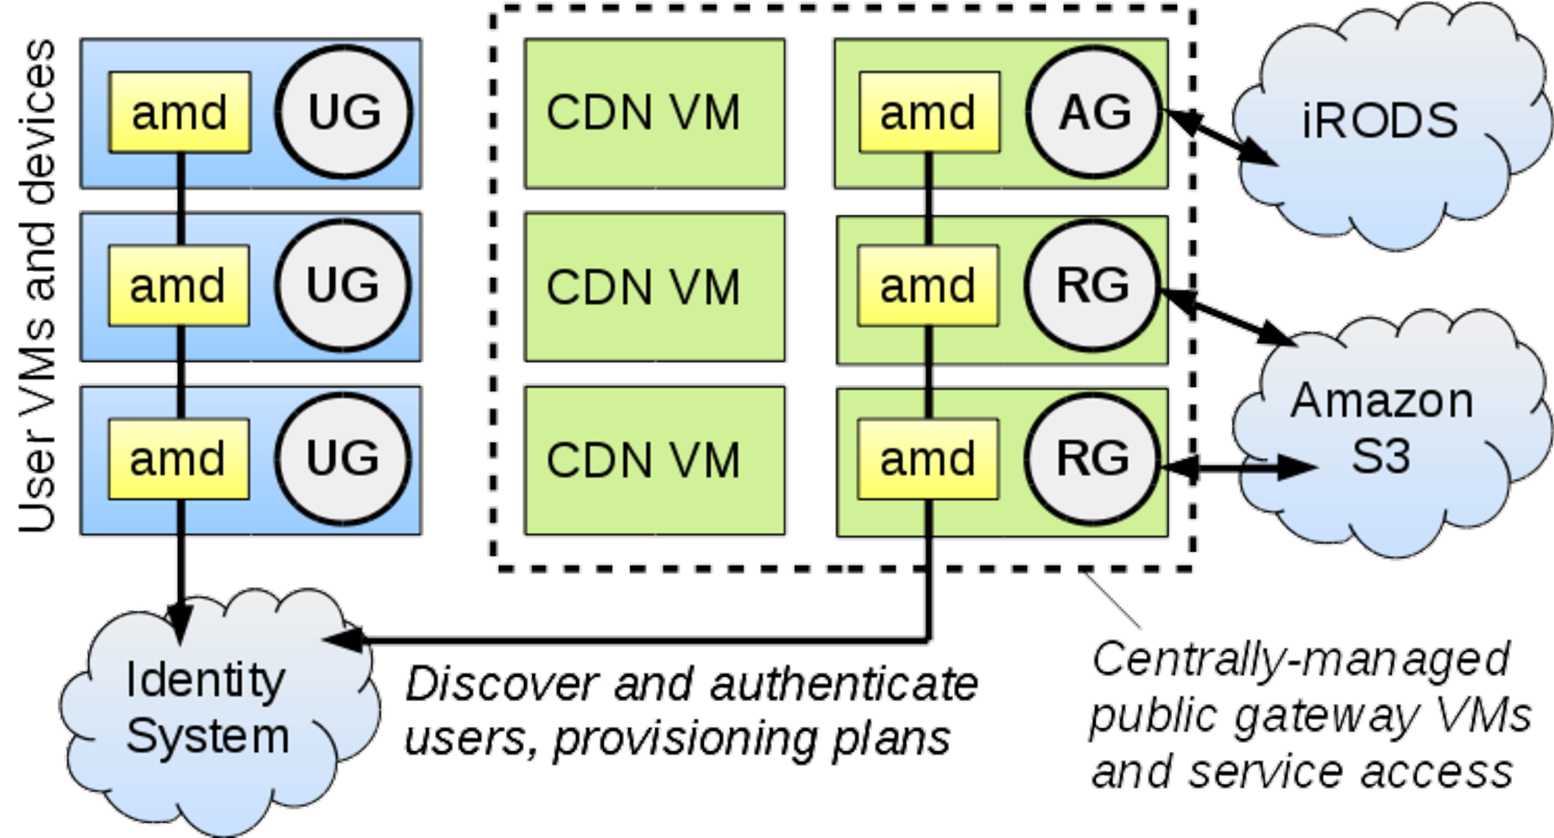
\includegraphics[width=0.47\textwidth]{figures/science-cloud}
\caption{\it Application 1: scientific storage.  A computing site gives users a
   space to run publicly-routable RGs and AGs to interface with their storage
   and existing datasets, and offers them a private CDN to enhance data
   availability.  To reduce the barriers to entry, the site could manage the
   RGs, AGs, and their storage logic on behalf of users, and simply bill them
   for their data consumed.  The automount client daemon (\texttt{amd}) manages
   each host's gateways.}
\label{fig:science-cloud}
\end{figure}


The first is a wide-area scientific data volume manager that spans
multiple administrative domains (Figure~\ref{fig:science-cloud}). The storage requirements are that
data is replicated to Amazon S3, and must be encrypted at rest and in transit.
Frequently request data must be cached in a private, shared CDN. The application
itself is concerned with translating user intentions via a GUI into requests to
the automount clients running on the user's VMs and devices. The RG logic required to
implement this system is only 150 lines of Python (to interface with S3) and the
UG logic is only 300 lines (to interface with the CDN and encrypt data).

The automount service and the self-sovereign identity service remove the need
for a dedicated configuration and key server.  Both the users and service
operators use a locally-hosted GUI tool to replicate and distribute new
provision plans via the externally-operated identity service.  Because each host knows
the username of its owner, its automount client automatically uses the latest
authentic configuration state to instantiate gateways.

\begin{figure}[t!]
\centering
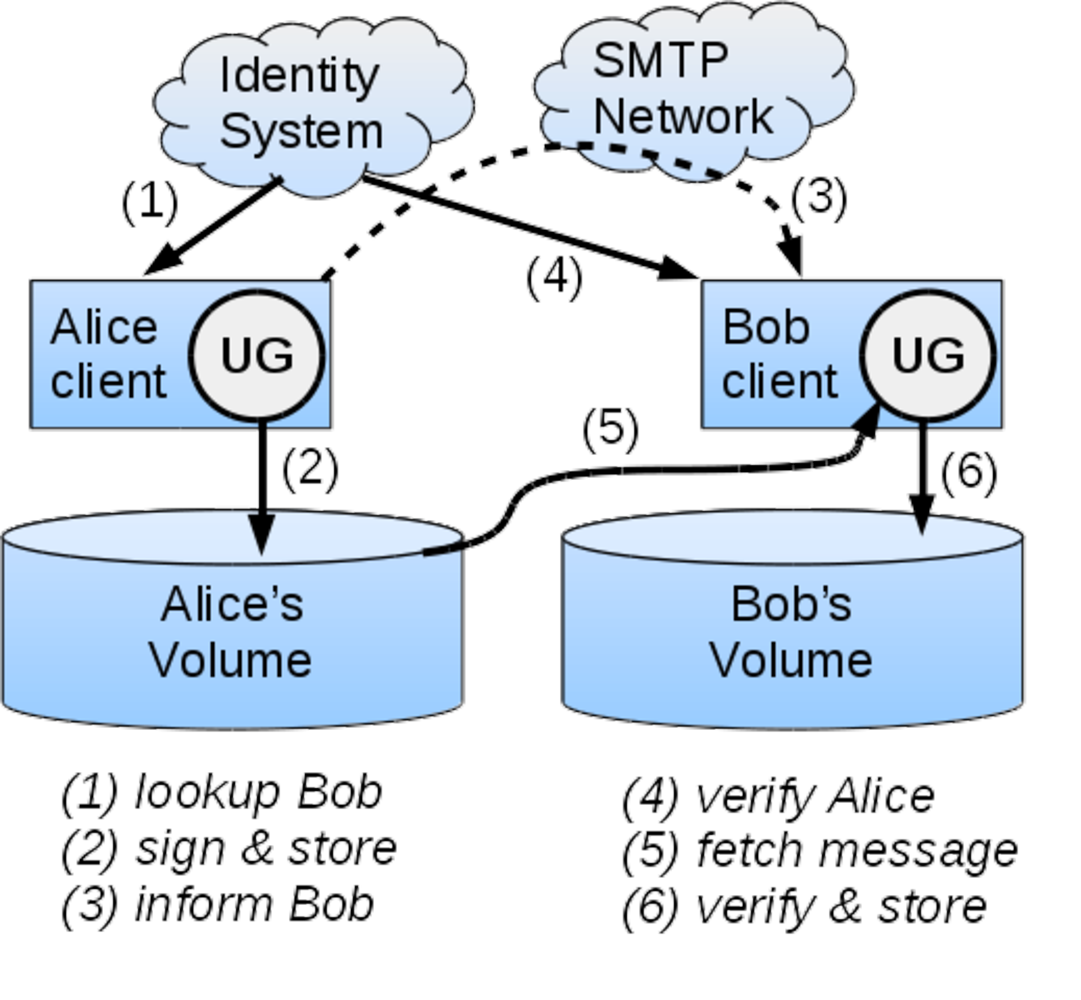
\includegraphics[width=0.47\textwidth]{figures/secure-mail}
\caption{\it Application 2: end-to-end secure webmail. Alice and Bob store
   signed encrypted messages to one another on their own volumes, and use a
   shared self-sovereign identity service to discover each other's public keys.
   They rely on the legacy SMTP network to inform one another when they have new
   mail.}
\label{fig:secure-mail}
\end{figure}

The second application implements PGP email without requiring users to interact
with PGP keys (Figure~\ref{fig:secure-mail}) or run their own mail servers.
To users, the system looks like a webmail. The application is
local HTTP proxy that serves the web application, and contains a UG to store the
inbox and outgoing mail in the user's volume. It uses the legacy SMTP
network to announce messages to recipients. This way, Bob's proxy will be
notified (via a signed SMTP message) that there is an encrypted message in
Alice's volume waiting for him, and will automatically fetch, authenticate,
decrypt, and serve it to him in his browser. The RG logic required to implement
this system is identical to that in the first application. The UG logic is about
1000 lines, to both interface with SMTP servers and additionally encrypt the
path to the message in the volume. It uses a self-sovereign identity system to discover Alice's and
Bob's keys.

\begin{figure}[t!]
\centering
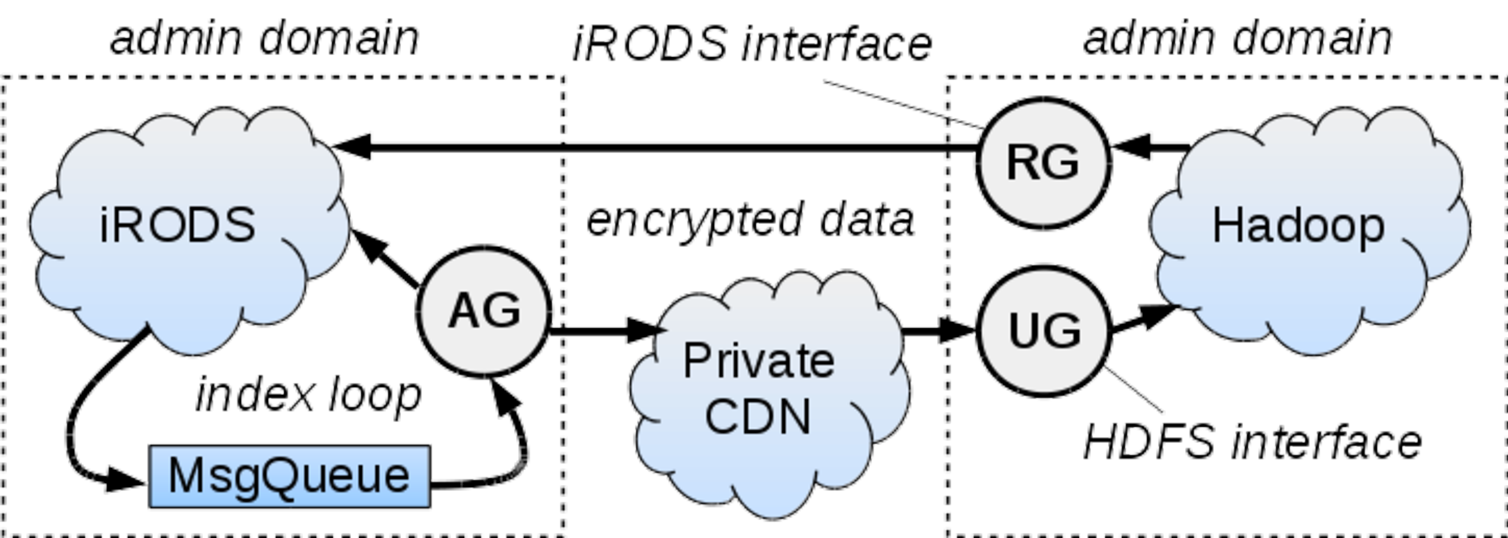
\includegraphics[width=0.47\textwidth]{figures/irods-hadoop}
\caption{\it Application 3: science site integrations.  Waskern enables external
   gateways to discover files in an intra-site iRODS deployment, where the
   site's AG serves to authenticate external requests on its behalf and serve
   data through a private CDN.  The private CDN removes the need to manually
   stage data at other sites, since hot data will be automatically cached
   locally.  The UG links remote Hadoop jobs to AG-served data, and provides
   Hadoop with a way to replicate results back to the original archive.}
\label{fig:irods-hadoop}
\end{figure}

The third application is a scientific storage service for making existing iRODS
deployments available to remote Hadoop jobs, without requiring manual data
staging and transfers (Figure~\ref{fig:irods-hadoop}). This application
uses an AG to import iRODS data into a volume. The private
CDN automatically stages data close to the remote Hadoop nodes, and remote UGs
ensure that any communication failures between the AG and iRODS get resolved
before a read completes. The remote Hadoop jobs copy back their new data into a
separate iRODS home directory via a local RG. The UG code in this application is
the same as in the first, but the AG code is about 1500 lines of Python and the RG
code is about 1000 lines.

This application removes two key barriers-to-entry for scientific computing.  By
relying on a commodity CDN and encrypting data in-flight, Waskern removes the
need for both dedicated science DMZ for hosting data and a dedicated service for
pushing it out to other science DMZs.  All the while, it remains compatible with
both iRODS and Hadoop, and ensures that Hadoop readers receive consistent data
regardless of the CDN's cache-control policies.

We are in the process of making these applications production-ready.  The
science-oriented applications are slated to link several universities' data repositories, and
the second application has already been demonstrated publicly and has received venture capital funding.

\subsection{Performance Overhead}

Our performance microbenchmark was intentionally conducted using only
freely-available Web services.  This is because we expect this to be the common
case for many users and developers, especially when trying out new applications
for the first time.  We ran our RG on a free-tier VM in Amazon
AWS~\cite{amazonaws}, we ran our MS as a free front-end service in Google
Appengine~\cite{google-appengine}, and we ran our UGs on local laptops behind
NATs.

\begin{figure}[t!]
\centering
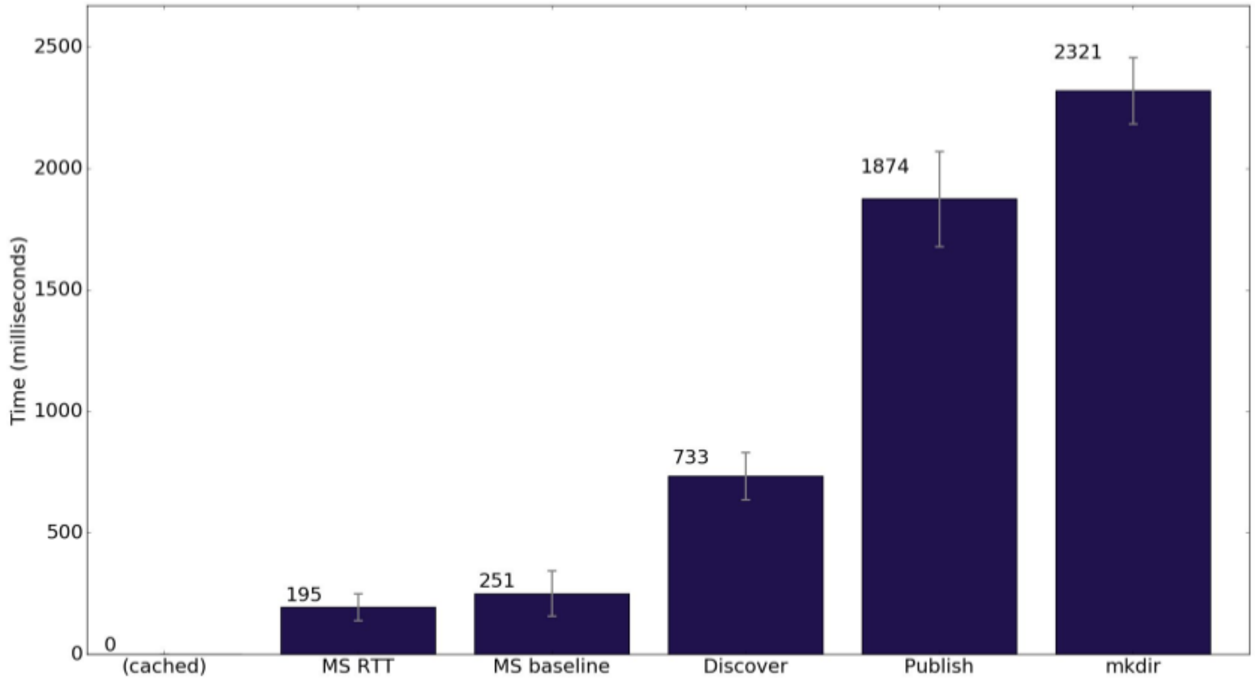
\includegraphics[width=0.47\textwidth]{figures/ms-performance}
\caption{\it MS performance in the free tier of Google Appengine for creating
   files (``Touch'') and directories (``Mkdir''), and reading them
   (``Stat'') when compared to baseline network performance (``Ping''). 
   Numbers are millisecond averages; error bars are standard deviations.}
\label{fig:ms-performance}
\end{figure}

Even with these operating constraints, Waskern's performance is comparable to
that of interacting with a Web application (Figure~\ref{fig:ms-performance}).
Looking up MS-cached metadata
(``Stat'') takes on average 733 milliseconds per request (n=50), caching
file data (``Touch'') takes on average 1874 milliseconds, and making a new
directory (``Mkdir'') takes on average 2321 milliseconds.  Making directories
requires instantiating extra indexing state within the MS, which accounts
for extra time it takes over caching only file state.  On average, 251
milliseconds (about 25\%) of these operations' time was spent routing the request to the Google
Appengine process (``Ping''), as measured by requesting an empty HTTP 200
response.

\begin{figure}[t!]
\centering
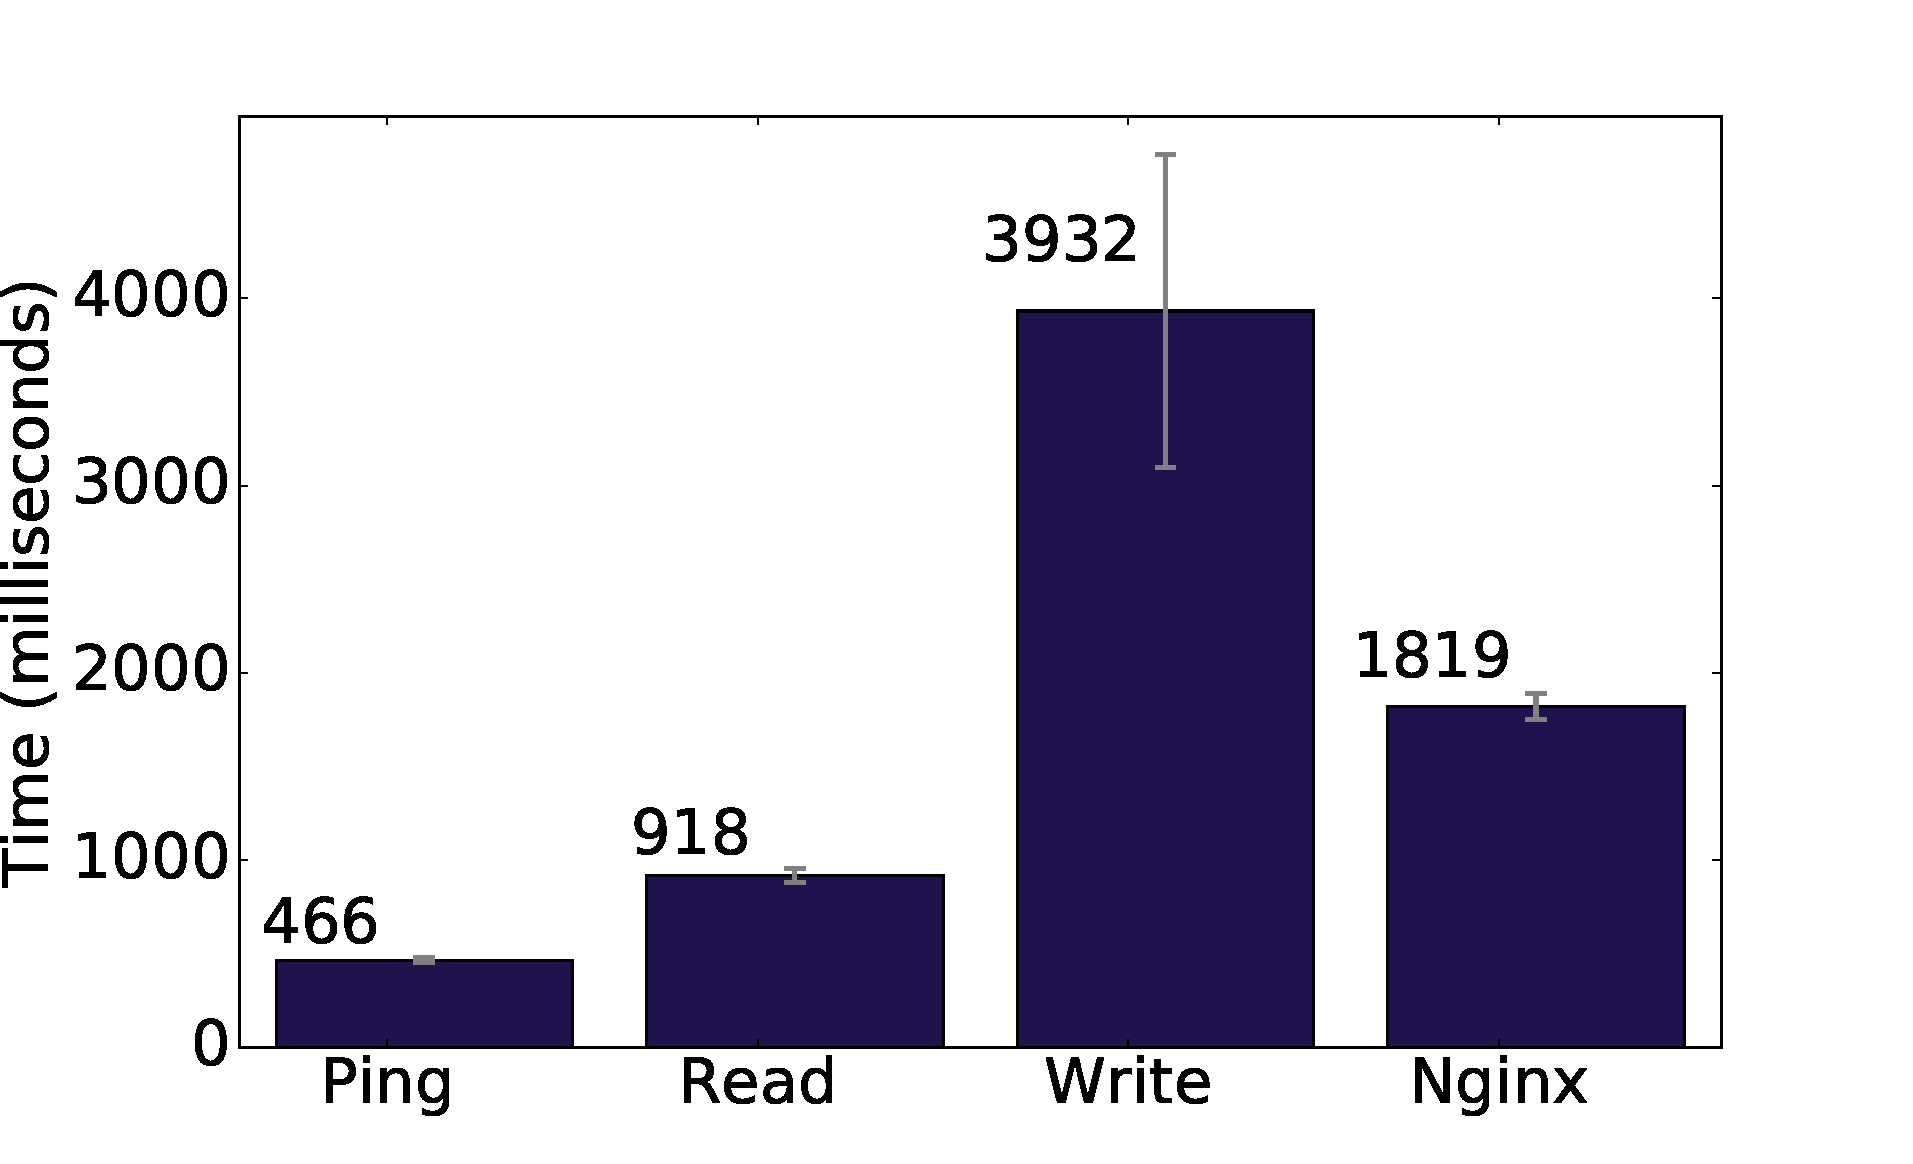
\includegraphics[width=0.47\textwidth]{figures/data-performance}
\caption{\it  UG/RG performance in the free tier of Amazon AWS.  A 10-block file
   with 10KB blocks was read and written 50 times each, using no-op storage
   logic.  Nginx \texttt{GET}s are slower than the RG's reads, even without caching.
   Write performance varies due to virtualized CPU and network-backed storage.
   Numbers are millisecond averages; error bars are standard deviations.}
\label{fig:data-performance}
\end{figure}

To measure the performance overhead of reading and writing data, we instantiated
a UG on a local laptop and an RG in the free tier in Amazon AWS.  We compared
its performance to Nginx~\cite{nginx}, a commonly-used high-performance Web
server (Figure~\ref{fig:data-performance}).  We used the UG to do whole-file
reads and writes a 10-block file with 10k blocks a total of 50 times.
The I/O flow processing logic in the RG simply read and
wrote chunks to local disk, and the UG's flow-processing simply
forwarded chunks to the RG.

We measured time on the UG.  For reads, this is the time between initiating the
read and completing it.  No data was cached between reads.  For writes, this is
the time between initiating the write, and completing both the write and then
subsequently ``\texttt{fsync()}''-ing the written chunks to the RG.

This test shows that interacting with an RG is comparable with interacting with Nginx.
Reading data is faster than GET'ing the equivalent data from Nginx,
since the RG has a shallower and less featureful HTTP GET path (based on
GNU libmicrohttpd~\cite{libmicrohttpd}).  Write performance varied widely because the VM's vCPU runs at a lower priority
than other tenant vCPUs, and its disk is based on networked-back storage with no
SLAs. 

In their current unoptimized state, interacting with Waskern volumes deployed to
free cloud services has comparable latency and bandwidth to interacting with a heavyweight
Web service.  We expect performance to improve after addressing some low-hanging
performance fruit.

% [note by illyoung: The same UG logic as in the first is used but I/O interface
% is exposed via RESTful using Node.js. Also, an application that translates
% Hadoop filesystem operations to the Waskern UG operations is implemented in
% Java.]

